%%%%%%%%%%%%%%%%%%%%%%%%%%%%%%%%%%%%%%%%%%%%%%%%%%%%%%%%%%%%%%%%%%%%%%%%%%%%%%%

\documentclass[a4paper,10pt]{llncs}

%%%%%%%%%%%%%%%%%%%%%%%%%%%%%%%%%%%%%%%%%%%%%%%%%%%%%%%%%%%%%%%%%%%%%%%%%%%%%%%

\usepackage[utf8x]{inputenc}
\usepackage{amssymb}
\usepackage{amsmath}
\usepackage{amsfonts}
\usepackage{graphicx}
%\usepackage{llncsdoc}
\usepackage[english]{babel}
\usepackage[ruled,vlined,linesnumbered]{algorithm2e}
\usepackage{algorithmic}
\usepackage{float}
\usepackage{todonotes}
\usepackage{subfigure}

\usepackage{tikz}
\usetikzlibrary{matrix, calc, arrows}

%%%%%%%%%%%%%%%%%%%%%%%%%%%%%%%%%%%%%%%%%%%%%%%%%%%%%%%%%%%%%%%%%%%%%%%%%%%%%%%

%%% 
%%% complexity.tex
%%% 

\usepackage{xspace}

%%% ----------------------------------------------------------------------
%%% complexity classes
%%% ----------------------------------------------------------------------

% TIME
\newcommand{\DTIMEX}{{\sf\bf DTIME}}
\newcommand{\DTIMEclass}{\DTIMEX\xspace}
\newcommand{\DTIME}{\DTIMEclass}
% NL class
\newcommand{\NLclassbase}{{\sf\bf NL}}
\newcommand{\NLclass}{\NLclassbase\xspace}
% P class
\newcommand{\Pclassbase}{{\sf\bf P}}
\newcommand{\Pclass}{\Pclassbase\xspace}
% NP class
\newcommand{\NPclassbase}{{\sf\bf NP}}
\newcommand{\NPclass}{\NPclassbase\xspace}
% coNP class
\newcommand{\coNPclassbase}{{\sf\bf coNP}}
\newcommand{\coNPclass}{\coNPclassbase\xspace}
% PSPACE class
\newcommand{\PSPACEclassbase}{{\sf\bf PSPACE}}
\newcommand{\PSPACEclass}{\PSPACEclassbase\xspace}
% MAXSNP class
\newcommand{\MaxSNPclassbase}{{\sf\bf MaxSNP}}
\newcommand{\MaxSNPclass}{\MaxSNPclassbase\xspace}
% MAXNP class
\newcommand{\MaxNPclassbase}{{\sf\bf MaxNP}}
\newcommand{\MaxNPclass}{\MaxNPclassbase\xspace}
% EPTAS class
\newcommand{\EPTASclassbase}{{\sf\bf EPTAS}}
\newcommand{\EPTASclass}{\EPTASclassbase\xspace}
% FPTAS class
\newcommand{\FPTASclassbase}{{\sf\bf FPTAS}}
\newcommand{\FPTASclass}{\FPTASclassbase\xspace}
% PTAS class
\newcommand{\PTASclassbase}{{\sf\bf PTAS}}
\newcommand{\PTASclass}{\PTASclassbase\xspace}
% APX class
\newcommand{\APXclassbase}{{\sf\bf APX}}
\newcommand{\APXclass}{\APXclassbase\xspace}
% log-APX class
\newcommand{\logAPXclassbase}{{\sf\bf log{\tt -}APX}}
\newcommand{\logAPXclass}{\logAPXclassbase\xspace}
% poly-APX class
\newcommand{\polyAPXclassbase}{{\sf\bf poly{\tt -}APX}}
\newcommand{\polyAPXclass}{\polyAPXclassbase\xspace}
% exp-APX class
\newcommand{\expAPXclassbase}{{\sf\bf exp{\tt -}APX}}
\newcommand{\expAPXclass}{\expAPXclassbase\xspace}
% NPO class
\newcommand{\NPOclassbase}{{\sf\bf NPO}}
\newcommand{\NPOclass}{\NPOclassbase\xspace}
% #P class
\newcommand{\sharpPclassbase}{\#{\sf\bf P}}
\newcommand{\sharpPclass}{\sharpPclassbase\xspace}
% FPT class
\newcommand{\FPTclassbase}{{\sf\bf FPT}}
\newcommand{\FPTclass}{\FPTclassbase\xspace}
% W class
\newcommand{\Wclassbase}[1]{{\sf\bf W[#1]}}
\newcommand{\Wclass}[1]{\Wclassbase{#1}\xspace}
% W class
\newcommand{\XPclassbase}{{\sf\bf XP}}
\newcommand{\XPclass}{\XPclassbase\xspace}
% WNL class
\newcommand{\WNLclassbase}{{\sf\bf WNL}}
\newcommand{\WNLclass}{\WNLclassbase\xspace}
% ZPP class
\newcommand{\ZPPclassbase}{{\sf\bf ZPP}}
\newcommand{\ZPPclass}{\ZPPclassbase\xspace}
% NPK class
\newcommand{\NPKclassbase}{{\sf\bf NPK}}
\newcommand{\NPKclass}{\NPKclassbase\xspace}
\newcommand{\NPKandclass}{\text{$\NPKclass_\text{and}$}\xspace}
\newcommand{\NPKzeroandclass}{\text{$\NPKclass^0_\text{and}$}\xspace}
\newcommand{\NPKorclass}{\text{$\NPKclass_\text{or}$}\xspace}
\newcommand{\NPKzeroorclass}{\text{$\NPKclass^0_\text{or}$}\xspace}

%%% ----------------------------------------------------------------------
%%% complete
%%% ----------------------------------------------------------------------

% keyword
\newcommand{\complete}{\text{-complete}}
% NL-complete
\newcommand{\NLcomplete}{\NLclassbase\complete\xspace}
\newcommand{\NLC}{\NLcomplete}
% P-complete
\newcommand{\Pcomplete}{\Pclassbase\complete\xspace}
\newcommand{\PC}{\Pcomplete}
% NP-complete
\newcommand{\NPcomplete}{\NPclassbase\complete\xspace}
\newcommand{\NPC}{\NPcomplete}
% coNP-complete
\newcommand{\coNPcomplete}{\coNPclassbase\complete\xspace}
\newcommand{\coNPC}{\coNPcomplete}
% PSPACE-complete
\newcommand{\PSPACEcomplete}{\PSPACEclassbase\complete\xspace}
\newcommand{\PSPACEC}{\PSPACEcomplete}
% MAXSNP-complete
\newcommand{\MaxSNPcomplete}{\MaxSNPclassbase\complete\xspace}
\newcommand{\MaxSNPC}{\MaxSNPcomplete}
% APX-complete
\newcommand{\APXcomplete}{\APXclassbase\complete\xspace}
\newcommand{\APXC}{\APXcomplete}
% #P-complete
\newcommand{\sharpPcomplete}{\sharpPclassbase\complete\xspace}
\newcommand{\sharpPC}{\sharpPcomplete}
% W[i]-complete
\newcommand{\Wcomplete}[1]{\Wclassbase{#1}\complete\xspace}
\newcommand{\WC}[1]{\Wcomplete{#1}}
% WNL-complete
\newcommand{\WNLcomplete}{\WNLclassbase\complete\xspace}
\newcommand{\WNLC}{\WNLcomplete}

%%% ----------------------------------------------------------------------
%%% hard
%%% ----------------------------------------------------------------------

% keyword
\newcommand{\hard}{\text{-hard}}
% NL-hard
\newcommand{\NLhard}{\NLclassbase\hard\xspace}
\newcommand{\NLH}{\NLhard}
% P-hard
\newcommand{\Phard}{\NPclassbase\hard\xspace}
\newcommand{\PH}{\Phard}
% NP-hard
\newcommand{\NPhard}{\NPclassbase\hard\xspace}
\newcommand{\NPH}{\NPhard}
% coNP-hard
\newcommand{\coNPhard}{\coNPclassbase\hard\xspace}
\newcommand{\coNPH}{\coNPhard}
% PSPACE-hard
\newcommand{\PSPACEhard}{\PSPACEclassbase\hard\xspace}
\newcommand{\PSPACEH}{\PSPACEhard}
% MAXSNP-hard
\newcommand{\MaxSNPhard}{\MaxSNPclassbase\hard\xspace}
\newcommand{\MaxSNPH}{\MaxSNPhard}
% APX-hard
\newcommand{\APXhard}{\APXclassbase\hard\xspace}
\newcommand{\APXH}{\APXhard}
% WNL-hard
\newcommand{\WNLhard}{\WNLclassbase\hard\xspace}
\newcommand{\WNLH}{\WNLhard}
% #P-hard
\newcommand{\sharpPhard}{\sharpPclassbase\hard\xspace}
\newcommand{\sharpPH}{\sharpPhard}
% W[i]-hard
\newcommand{\Whard}[1]{\Wclassbase{#1}\hard\xspace}
\newcommand{\WH}[1]{\Whard{#1}}

%%% ----------------------------------------------------------------------
%%% hardness
%%% ----------------------------------------------------------------------

% keyword
\newcommand{\hardness}{\text{-hardness}}
% NP-hardness
\newcommand{\NPhardness}{\NPclassbase\hardness\xspace}
% APX-hardness
\newcommand{\APXhardness}{\APXclassbase\hardness\xspace}
% W[i]-hardness
\newcommand{\Whardness}[1]{\Wclassbase{#1}\hardness\xspace}
% WNL-hardness
\newcommand{\WNLhardness}{\WNLclassbase\hardness\xspace}

%%% ----------------------------------------------------------------------
%%% completeness
%%% ----------------------------------------------------------------------

% keyword
\newcommand{\completeness}{\text{-completeness}}
% NL-completeness
\newcommand{\NLcompleteness}{\NLclassbase\completeness\xspace}
% P-completeness
\newcommand{\Pcompleteness}{\NPclassbase\completeness\xspace}
% NP-completeness
\newcommand{\NPcompleteness}{\NPclassbase\completeness\xspace}
% APX-completeness
\newcommand{\APXcompleteness}{\APXclassbase\completeness\xspace}
% #P-completeness
\newcommand{\sharpPcompleteness}{\sharpPclassbase\completeness\xspace}
% W[i]-hard
\newcommand{\Wcompleteness}[1]{\W{#1}-\completeness\xspace}

%%% ----------------------------------------------------------------------
%%% reduction
%%% ----------------------------------------------------------------------

\newcommand{\reduction}{reduction}
\newcommand{\reductions}{reductions}
\newcommand{\reductible}{reductible}

\newcommand{\APTypeReduction}{AP}
\newcommand{\PTASTypeReduction}{PTAS}
\newcommand{\LTypeReduction}{L}
\newcommand{\ETypeReduction}{E}
\newcommand{\fptTypeReduction}{fpt}
\newcommand{\pptTypeReduction}{ptp}

% AP-reduction
\newcommand{\APreduction}{\APTypeReduction-\reduction\xspace}
\newcommand{\APreductions}{\APTypeReduction-\reductions\xspace}
\newcommand{\APreductible}{\APTypeReduction-\reductible\xspace}

% PTAS-reduction
\newcommand{\PTASeduction}{\PTASTypeReduction-\reduction\xspace}
\newcommand{\PTASreductions}{\PTASTypeReduction-\reductions\xspace}
\newcommand{\PTASreductible}{\PTASTypeReduction-\reductible\xspace}

% L-reduction
\newcommand{\Lreduction}{\LTypeReduction-\reduction\xspace}
\newcommand{\Lreductions}{\LTypeReduction-\reductions\xspace}
\newcommand{\Lreductible}{\LTypeReduction-\reductible\xspace}

% E-reduction
\newcommand{\Ereduction}{\ETypeReduction-\reduction\xspace}
\newcommand{\Ereductions}{\ETypeReduction-\reductions\xspace}
\newcommand{\Ereductible}{\ETypeReduction-\reductible\xspace}

% fpt-reduction
\newcommand{\fptreduction}{\fptTypeReduction-\reduction\xspace}
\newcommand{\fptreductions}{\fptTypeReduction-\reductions\xspace}
\newcommand{\fptreductible}{\fptTypeReduction-\reductible\xspace}

% ptp-reduction
\newcommand{\ptpreduction}{\ptpTypeReduction-\reduction\xspace}
\newcommand{\ptpreductions}{\ptpTypeReduction-\reductions\xspace}
\newcommand{\ptpreductible}{\ptpTypeReduction-\reductible\xspace}

% symbols
\DeclareMathOperator{\APreduce}{\text{$\leq_{\text{\APTypeReduction}}$}}
\DeclareMathOperator{\PTASreduce}{\text{$\leq_{\text{\PTASTypeReduction}}$}}
\DeclareMathOperator{\Lreduce}{\text{$\leq_{\text{\LTypeReduction}}$}}
\DeclareMathOperator{\Ereduce}{\text{$\leq_{\text{\ETypeReduction}}$}}
\DeclareMathOperator{\fptreduce}{\text{$\leq_{\text{\fptTypeReduction}}$}}
\DeclareMathOperator{\ptpreduce}{\text{$\leq_{\text{\fptTypeReduction}}$}}

%% 
%% Approximation
%%
\DeclareMathOperator{\poly}{poly}
\DeclareMathOperator{\POLY}{poly}
\DeclareMathOperator{\SIZE}{size}
\newcommand{\sol}{{\sf sol}\xspace}
\newcommand{\PB}[1]{\textsf{\scshape{#1}}}
\newcommand{\OPTname}{opt}
\newcommand{\OPT}{\text{$\mathsf{\bf \OPTname}$}}
\newcommand{\OPTpb}[1]{\text{$\mathsf{\OPTname}_{\PB{#1}}$}}
\newcommand{\ALGO}[1]{\textbf{\ttfamily\sf #1}}
\newcommand{\Approxname}{Approx}
\newcommand{\APPROX}[1]{\text{$\ALGO{\Approxname}_{\,\PB{#1}}$}}
\newcommand{\PCP}{{\sf\bf PCP}\xspace}

%%
%% Problem Definition
%%
\newcommand{\PbDef}[3]{%
\begin{center}
  \begin{tabular}{l}%
    \shadowbox{%
    \begin{minipage}[c]{.9\textwidth}
      \smallskip%
      \par\noindent%
      {#1}%
      \smallskip
      \par\noindent%
      $\bullet$
      \textbf{\textsf{Input}}~: #2% 
      \medskip
      \par\noindent%
      $\bullet$
      \textbf{\textsf{Question}}~:
      #3% 
      \smallskip%
      \par\noindent%
    \end{minipage}
  }% end shadowbox
  \end{tabular}%
\end{center}
}%
\newcommand{\PbDefinition}{\PbDef}

%%
%% Problem (Input + Output) Definition
%%
\newcommand{\PbInputOutputDef}[3]{%
\begin{center}
  \begin{tabular}{l}%
    \shadowbox{%
    \begin{minipage}[c]{.9\textwidth}
      \smallskip%
      \par\noindent%
      \PB{#1}%
      \medskip%
      \par\noindent%
      $\bullet$
      \textbf{\textsf{Input}}~: #2% 
      \medskip
      \par\noindent%
      $\bullet$
      \textbf{\textsf{Output}}~:
      #3% 
      \smallskip%
      \par\noindent%
    \end{minipage}
  }% end shadowbox
  \end{tabular}%
\end{center}
}%
\newcommand{\PbInputOutputDefinition}{\PbInputOutputDef}


%%
%% Optimization Problem Definition
%%

\newcommand{\OptPbDefinition}[4]{%
\begin{center}
  \begin{tabular}{l}%
    \shadowbox{%
    \begin{minipage}[c]{.9\textwidth}
      \par\noindent%
      \shadowbox{#1}%
      \par\noindent%
      $\bullet$
      \textbf{\textsf{Input}}~: #2% 
      \par\noindent%
      $\bullet$
      \textbf{\textsf{Solution}}~: #3%  
      \par\noindent%
      $\bullet$
      \textbf{\textsf{Measure}}~: #4% 
      \par\noindent%
    \end{minipage}
    }% end shadowbox
  \end{tabular}%
\end{center}
}%

%%
%% Parameterized Problem Definition
%%
\newcommand{\ParamPbDefinition}[4]{%
\begin{center}
  \begin{tabular}{l}%
    %\shadowbox{%
    \begin{minipage}[c]{.95\textwidth}
      % \smallskip%
      \par\noindent%
      #1%
      % \smallskip%
      \par\noindent%
      \textbf{\textsf{Input}}~: #2% 
      % \smallskip
      \par\noindent%
      \textbf{\textsf{Question}}~: #3%  
      % \smallskip
      \par\noindent%
      \textbf{\textsf{Parameter}}~: #4% 
      %\smallskip%
      \par\noindent%
    \end{minipage}
  %}% end shadowbox
  \end{tabular}%
\end{center}
}%
\newcommand{\ParamPbDefinitionTwo}[5]{%
\begin{center}
  \begin{tabular}{l}%
    \shadowbox{%
    \begin{minipage}[c]{.9\textwidth}
      \smallskip%
      \par\noindent%
      \shadowbox{#1}%
      \medskip%
      \par\noindent%
      $\bullet$
      \textbf{\textsf{Input}}~: #2% 
%      \medskip
      \par\noindent%
      $\bullet$
      \textbf{\textsf{Parameter}}~: #3% 
 %     \medskip
      \par\noindent%
      $\bullet$
      \textbf{\textsf{Parameter}}~: #4% 
      \medskip
      \par\noindent%
      $\bullet$
      \textbf{\textsf{Question}}~: #5%  
      \smallskip%
      \par\noindent%
    \end{minipage}
    }% end shadowbox
  \end{tabular}%
\end{center}
}%
\newcommand{\ParamPbDefinitionThree}[6]{%
\begin{center}
  \begin{tabular}{l}%
    \shadowbox{%
    \begin{minipage}[c]{.9\textwidth}
      \smallskip%
      \par\noindent%
      \shadowbox{#1}%
      \medskip%
      \par\noindent%
      $\bullet$
      \textbf{\textsf{Input}}~: #2% 
%      \medskip
      \par\noindent%
      $\bullet$
      \textbf{\textsf{Parameter}}~: #3% 
%      \medskip
      \par\noindent%
      $\bullet$
      \textbf{\textsf{Parameter}}~: #4% 
%      \medskip
      \par\noindent%
      $\bullet$
      \textbf{\textsf{Parameter}}~: #5%  
      \medskip
      \par\noindent%
      $\bullet$
      \textbf{\textsf{Question}}~: #6%  
      \smallskip%
      \par\noindent%
    \end{minipage}
    }% end shadowbox
  \end{tabular}%
\end{center}
}%
\newcommand{\ParamPbDefinitionFour}[7]{%
\begin{center}
  \begin{tabular}{l}%
    \shadowbox{%
    \begin{minipage}[c]{.9\textwidth}
      \smallskip%
      \par\noindent%
      \shadowbox{#1}%
      \medskip%
      \par\noindent%
      $\bullet$
      \textbf{\textsf{Input}}~: #2% 
%      \medskip
      \par\noindent%
      $\bullet$
      \textbf{\textsf{Parameter}}~: #3% 
%      \medskip
      \par\noindent%
      $\bullet$
      \textbf{\textsf{Parameter}}~: #4% 
%      \medskip
      \par\noindent%
      $\bullet$
      \textbf{\textsf{Parameter}}~: #5%  
%      \medskip
      \par\noindent%
    $\bullet$
      \textbf{\textsf{Parameter}}~: #6%  
      \medskip
      \par\noindent%
      $\bullet$
      \textbf{\textsf{Question}}~: #7%  
      \smallskip%
      \par\noindent%
    \end{minipage}
    }% end shadowbox
  \end{tabular}%
\end{center}
}%
\newcommand{\ParamPbDefinitionFive}[8]{%
\begin{center}
  \begin{tabular}{l}%
    \shadowbox{%
    \begin{minipage}[c]{.9\textwidth}
      \smallskip%
      \par\noindent%
      \shadowbox{#1}%
      \medskip%
      \par\noindent%
      $\bullet$
      \textbf{\textsf{Input}}~: #2% 
%      \medskip
      \par\noindent%
      $\bullet$
      \textbf{\textsf{Parameter}}~: #3% 
%      \medskip
      \par\noindent%
      $\bullet$
      \textbf{\textsf{Parameter}}~: #4% 
%      \medskip
      \par\noindent%
      $\bullet$
      \textbf{\textsf{Parameter}}~: #5%  
%      \medskip
      \par\noindent%
    $\bullet$
      \textbf{\textsf{Parameter}}~: #6%  
%      \medskip
      \par\noindent%
    $\bullet$
      \textbf{\textsf{Parameter}}~: #7%  
      \medskip
      \par\noindent%
      $\bullet$
      \textbf{\textsf{Question}}~: #8%  
      \smallskip%
      \par\noindent%
    \end{minipage}
    }% end shadowbox
  \end{tabular}%
\end{center}
}%
\newcommand{\ParamPbDefinitionSix}[9]{%
\begin{center}
  \begin{tabular}{l}%
    \shadowbox{%
    \begin{minipage}[c]{.9\textwidth}
      \smallskip%
      \par\noindent%
      \shadowbox{#1}%
      \medskip%
      \par\noindent%
      $\bullet$
      \textbf{\textsf{Input}}~: #2% 
%      \medskip
      \par\noindent%
      $\bullet$
      \textbf{\textsf{Parameter}}~: #3% 
%      \medskip
      \par\noindent%
      $\bullet$
      \textbf{\textsf{Parameter}}~: #4% 
%      \medskip
      \par\noindent%
      $\bullet$
      \textbf{\textsf{Parameter}}~: #5%  
%      \medskip
      \par\noindent%
      $\bullet$
      \textbf{\textsf{Parameter}}~: #6%  
%      \medskip
      \par\noindent%
      $\bullet$
      \textbf{\textsf{Parameter}}~: #7%  
%      \medskip
      \par\noindent%
      $\bullet$
      \textbf{\textsf{Parameter}}~: #8%  
      \medskip
      \par\noindent%
      $\bullet$
      \textbf{\textsf{Question}}~: #9%  
      \smallskip%
      \par\noindent%
    \end{minipage}
    }% end shadowbox
  \end{tabular}%
\end{center}
}%




%%%%%%%%%%%%%%%%%%%%%%%%%%%%%%%%%%%%%%%%%%%%%%%%%%%%%%%%%%%%%%%%%%%%%%%%%%%%%%%

% \renewcommand{\floatpagefraction}{.9}
% \renewcommand{\textfraction}{.1}

%%%%%%%%%%%%%%%%%%%%%%%%%%%%%%%%%%%%%%%%%%%%%%%%%%%%%%%%%%%%%%%%%%%%%%%%%%%%%%%

\DeclareMathOperator{\LEFT}{\ell}
\DeclareMathOperator{\RIGHT}{r}
\DeclareMathOperator{\QQ}{\mathbb{Q}}
\DeclareMathOperator{\STD}{\mathrm{std}}
\DeclareMathOperator{\SHUFFLE}{\bullet}

%%%%%%%%%%%%%%%%%%%%%%%%%%%%%%%%%%%%%%%%%%%%%%%%%%%%%%%%%%%%%%%%%%%%%%%%%%%%%%%

\makeatletter
\newcommand{\pushright}[1]{\ifmeasuring@#1\else\omit\hfill$\displaystyle#1$\fi\ignorespaces}
\newcommand{\pushleft}[1]{\ifmeasuring@#1\else\omit$\displaystyle#1$\hfill\fi\ignorespaces}
\makeatother

%%%%%%%%%%%%%%%%%%%%%%%%%%%%%%%%%%%%%%%%%%%%%%%%%%%%%%%%%%%%%%%%%%%%%%%%%%%%%%%

\begin{document}

%%%%%%%%%%%%%%%%%%%%%%%%%%%%%%%%%%%%%%%%%%%%%%%%%%%%%%%%%%%%%%%%%%%%%%%%%%%%%%%

\title{%
Unshuffling Permutations}%

\author{%
  Samuele Giraudo\inst{1} \and
  St\'ephane Vialette\inst{1}
}% end author
\institute{%
  Universit\'e Paris-Est, LIGM (UMR 8049), CNRS, UPEM, ESIEE Paris, ENPC,
  F-77454, Marne-la-Vallée, France\\
  \email{samuele.giraudo@univ-mlv.fr} \\
  \email{vialette@univ-mlv.fr}
}% end institute
\date{\today}

\maketitle

%%%%%%%%%%%%%%%%%%%%%%%%%%%%%%%%%%%%%%%%%%%%%%%%%%%%%%%%%%%%%%%%%%%%%%%%%%%%%%%

\begin{abstract}
bla bla bla \ldots
\end{abstract}

%%%%%%%%%%%%%%%%%%%%%%%%%%%%%%%%%%%%%%%%%%%%%%%%%%%%%%%%%%%%%%%%%%%%%%%%%%%%%%%

%%
%%
%% ---- Introduction ----
%%
\section{Introduction}
\label{section:Introduction}


%%%%%%%%%%%%%%%%%%%%%%%%%%%%%%%%%%%%%%%%%%%%%%%%%%%%%%%%%%%%%%%%%%%%%%%%%%%%%%%

%%
%% ---- Notations ----
%%
\section{Notations}
\label{section:Notations}

% Définir :
% - ensemble $S$
% - standardisation $\STD$
% - notation $\pi_{|P}$ et $\pi_{|\bar P}$
% - notation $\pi^\sim$ (miroir)
% - notation $\bar \pi$ (complémentaire)
% - notation $\bar ^{-1}$ (inverse)

%%%%%%%%%%%%%%%%%%%%%%%%%%%%%%%%%%%%%%%%%%%%%%%%%%%%%%%%%%%%%%%%%%%%%%%%%%%%%%%

%%
%% ---- Algebraic issues ----
%%
\section{Algebraic issues}
\label{section:Algebraic issues}
Let use denote by $\QQ[S]$ the linear span of all permutations. We shall
define on this space a kind of shuffle product. For this purpose, we
first define a linear coproduct $\Delta$ on $\QQ[S]$ satisfying for
any permutation $\pi$,
\begin{equation} \label{equ:unshuffling_coproduct}
    \Delta(\pi) =
    \sum_{P \subseteq [|\pi|]}
    \STD\left(\pi_{|P}\right) \otimes \STD\left(\pi_{|\bar P}\right).
\end{equation}
We call $\Delta$ the {\em unshuffling coproduct of permutations}. For
instance,
\begin{equation}
    \Delta(213) =
    \epsilon \otimes 213 + 2. 1 \otimes 12 +
    1 \otimes 21 + 2. 12 \otimes 1 + 21 \otimes 1 + 213 \otimes \epsilon,
\end{equation}
\begin{equation}
    \Delta(1234) =
    \epsilon \otimes 1234 + 4. 1 \otimes 123 + 6. 12 \otimes 12 +
    4. 123 \otimes 1 + 1234 \otimes \epsilon,
\end{equation}
\begin{equation}\begin{split} \label{equ:example_unshuffling_coproduct}
    \Delta(1432) & =
    \epsilon \otimes 1432 + 3. 1 \otimes 132 + 1 \otimes 321 +
    3. 12 \otimes 21 \\ & + 3. 21 \otimes 12 + 3. 132 \otimes 1 +
    321 \otimes 1 + 1432 \otimes \epsilon.
\end{split}\end{equation}
\medskip

As any coproduct, $\Delta$ leads to the definition of a product obtained
by duality in the following way. From~\eqref{equ:unshuffling_coproduct},
for any permutation $\pi$, we have
\begin{equation}
    \Delta(\pi) =
    \sum_{\sigma, \nu \in S} \lambda_{\sigma, \nu}^{(\pi)} \;
    \sigma \otimes \nu,
\end{equation}
where the $\lambda_{\sigma, \nu}^{(\pi)}$ are nonnegative integers. Now,
by definition of duality, the dual product of $\Delta$ denoted by
$\SHUFFLE$ is a linear binary product on $\QQ[S]$. It satisfies, for any
permutations
$\sigma$ and $\nu$,
\begin{equation}
    \sigma \SHUFFLE \nu =
    \sum_{\pi \in S}
    \lambda_{\sigma, \nu}^{(\pi)} \; \pi.
\end{equation}
We call $\SHUFFLE$ the {\em shuffle product of permutations}. For
instance,
\begin{equation}\begin{split} \label{equ:example_shuffle_product}
    12 \SHUFFLE 21 & =
    1243 + 1324 + 2.1342 + 2.1423 + 3.1432 + 2134 + 2.2314 \\
    & + 3.2341 + 2413 + 2.2431 + 2.3124 + 3142 + 3.3214 + 2.3241 \\
    & + 3421 + 3.4123 + 2.4132 + 2.4213 + 4231 + 4312.
\end{split}\end{equation}
Observe that the coefficient $3$ of the permutation $1432$
in~\eqref{equ:example_shuffle_product} comes from the fact that the
coefficient of the tensor $12 \otimes 21$ is $3$
in~\eqref{equ:example_unshuffling_coproduct}.
\medskip

We say that a permutation $\pi$ {\em appears} in the shuffle
$\sigma \SHUFFLE \nu$ of two permutations $\sigma$ and $\nu$ if the
coefficient $\lambda_{\sigma, \nu}^{(\pi)}$ is different from zero.
Besides, a permutation $\pi$ is a {\em square} if there is a permutation
$\sigma$ such that $\pi$ appears in $\sigma \SHUFFLE \sigma$.
Equivalently, $\pi$ is a square if in the expansion of $\Delta(\pi)$,
there is a tensor $\sigma \otimes \sigma$ with a nonzero coefficient.
\medskip

\begin{proposition}
    The shuffle product $\SHUFFLE$ of permutations is associative and
    commutative.
\end{proposition}
\begin{proof}

\end{proof}
\medskip

\begin{proposition}
    If $\pi$ is a square permutation, then $\pi^\sim$, $\bar \pi$,
    and $\pi^{-1}$ are square.
\end{proposition}
\begin{proof}

\end{proof}
\medskip

%%%%%%%%%%%%%%%%%%%%%%%%%%%%%%%%%%%%%%%%%%%%%%%%%%%%%%%%%%%%%%%%%%%%%%%%%%%%%%%

%%
%% ---- Algorithmic issues ----
%%
\section{Algorithmic issues}
\label{section:Algorithmic issues}


\begin{proposition}
Let $\pi \in S_{2n}$.
Then,
$\pi$ is the union of two order-isomorphic pattern
if and only if
there exists a perfect containment-free mathing
$\mathcal{M}$ of $G_\pi$ such that
$\LEFT(\mathcal{M}) \simeq \RIGHT(\mathcal{M})$.
\end{proposition}

\begin{proposition}
Deciding whether a permutation is the union of two
order-isomorphic pattern is \NPC.
\end{proposition}


\begin{align*}
N_4 &= 2(2n + k + 2) + 1  = 4n + 2k + 5 \\
N_3 &= 2(2N_4 + 2n + 2k + 4) + 1 = 20n + 12k + 9 \\
N_2 &= 2(2N_3 + 2n + 2k + 4) + 1 \\
N_1 &= 2(2N_2 + 2n + 2k + 4) + 1\text{.}
\end{align*}

\begin{align*}
\sigma'  &= ((k+1) \; \sigma \; (k+2)) \; [2N_2 + N_4 + 2n + k + 2] \\
\pi'     &= ((n+1) \; \pi \; (n+2)) \; [2N_2 + N_4 + n + k + 2] \\
\sigma'' &= \sigma \; [2N_2 + N_4] \\
\pi''    &= \pi \; [2N_2 + N_4 + k] \\
\nu_1    &= \nearrow_{N_1} \; [2N_2 + 2N_3 + 2N_4 + 2n + 2k + 4] \\
\nu'_1   &= \nearrow_{N_1} \; [N_1 + 2N_2 + 2N_3 + 2N_4 + 2n + 2k + 4] \\
\nu_2    &= \nearrow_{N_2} \; [N_2] \\
\nu'_2   &= \searrow_{N_2} \\
\nu_3    &= \nearrow_{N_3} \; [2N_2 + 2N_4 + 2n + 2k + 4] \\
\nu'_3   &= \nearrow_{N_3} \; [2N_2 + N_3 + 2N_4 + 2n + 2k + 4] \\
\nu_4    &= \searrow_{N_4} \; [2N_2 + N_4 + 2n + 2k + 4] \\
\nu'_4   &= \searrow_{N_4} \; [2N_2]
\end{align*}

$$
\mu
=
\nu_1 \; \nu_2 \; \nu'_1 \; \nu_3 \; \sigma' \; \nu_4 \; \nu'_3 \; \pi' \; \nu'_4 \; \pi'' \; \sigma''
$$

\begin{claim}
  \label{claim:no nu_1 - nu_1 edge}
  There is no $(\nu_1, \nu_2)$-edge in $\mathcal{M}$.
\end{claim}

\begin{proof}[of Claim~\ref{claim:no nu_1 - nu_1 edge}]
Suppose, aiming at a contradiction that there exists
a $(\nu_1, \nu_2)$-edge in $\mathcal{M}$.

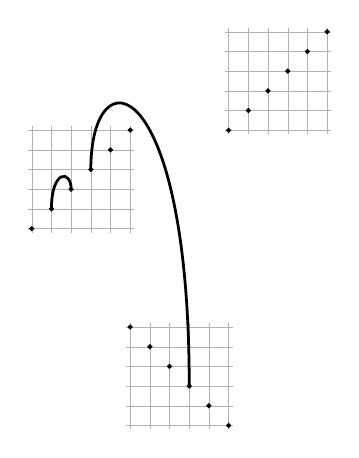
\begin{tikzpicture}
  [scale=0.25]
  % nu_1
  \draw[step=1cm,black!30,ultra thin,fill=black!10] (-0.2,9.8) grid (5.2,15.2);
  \foreach \x/\y in {0/10,1/11,2/12,3/13,4/14,5/15} {
      \draw [fill=black] (\x,\y) circle (0.1);
  }
  % nu_4
  \draw[step=1cm,black!30,ultra thin,fill=black!10] (4.8,-0.2) grid (10.2,5.2);
  \foreach \x/\y in {5/5,6/4,7/3,8/2,9/1,10/0} {
      \draw [fill=black] (\x,\y) circle (0.1);
  }
  % nu'_1
  \draw[step=1cm,black!30,ultra thin,fill=black!10] (9.8,14.8) grid (15.2,20.2);
  \foreach \x/\y in {10/15,11/16,12/17,13/18,14/19,15/20} {
      \draw [fill=black] (\x,\y) circle (0.1);
  }
  % edges
  \draw [line width=1pt]
  (1,11) .. controls +(0,2) and +(0,1) .. (2,12);
  \draw [line width=1pt]
  (3,13) .. controls +(0,6) and +(0,16) .. (8,2);
\end{tikzpicture}
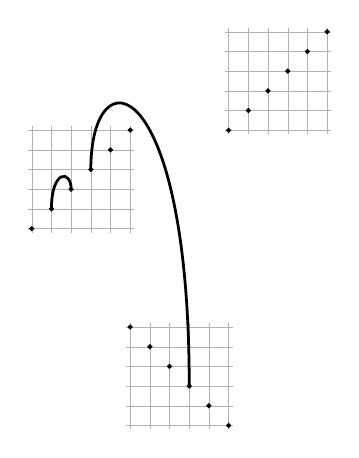
\begin{tikzpicture}
  [scale=0.25]
  % nu_1
  \draw[step=1cm,black!30,ultra thin,fill=black!10] (-0.2,9.8) grid (5.2,15.2);
  \foreach \x/\y in {0/10,1/11,2/12,3/13,4/14,5/15} {
      \draw [fill=black] (\x,\y) circle (0.1);
  }
  % nu_4
  \draw[step=1cm,black!30,ultra thin,fill=black!10] (4.8,-0.2) grid (10.2,5.2);
  \foreach \x/\y in {5/5,6/4,7/3,8/2,9/1,10/0} {
      \draw [fill=black] (\x,\y) circle (0.1);
  }
  % nu'_1
  \draw[step=1cm,black!30,ultra thin,fill=black!10] (9.8,14.8) grid (15.2,20.2);
  \foreach \x/\y in {10/15,11/16,12/17,13/18,14/19,15/20} {
      \draw [fill=black] (\x,\y) circle (0.1);
  }
  % edges
  \draw [line width=1pt]
  (1,11) .. controls +(0,2) and +(0,1) .. (2,12);
  \draw [line width=1pt]
  (3,13) .. controls +(0,6) and +(0,16) .. (8,2);
\end{tikzpicture}
\qed
\end{proof}

\begin{claim}
There is at least one $(\nu_1, \nu'_1)$-edge in $\mathcal{M}$.
\end{claim}

\begin{figure}[t!]
  \centering
  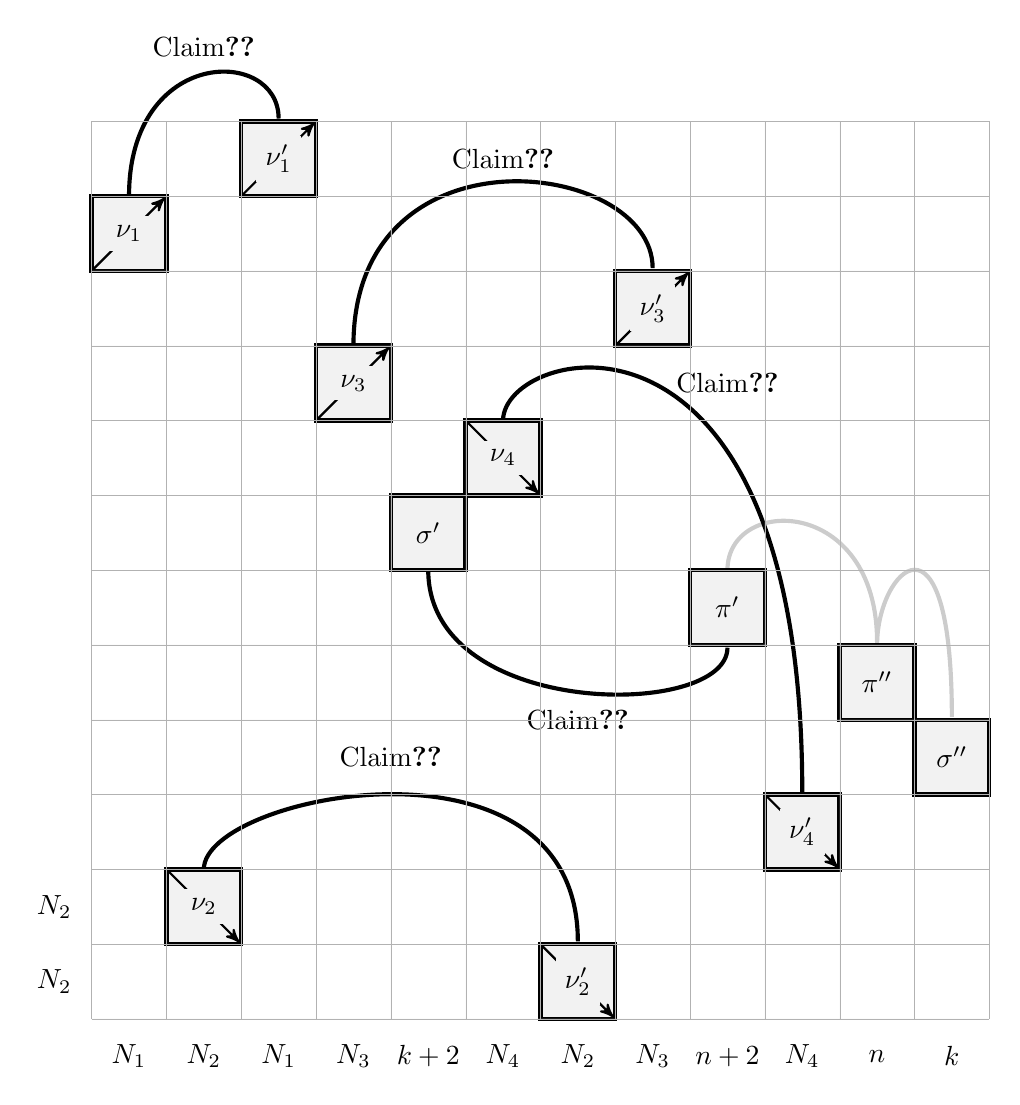
\begin{tikzpicture}[
    scale=.95,
    >=stealth',
    shorten >=1pt,
    main node/.style={align=center},
    cell/.style={draw,ultra thick,fill=black!5},
    structure link/.style={line width=1.5pt},
    pattern link/.style={line width=1.5pt,black!20},
    monotone/.style={->,thick}
    ]
    % edges
    % pi 1 - pi 2
    \draw [pattern link] (8.5,6) .. controls +(0,1) and +(0,2) .. (10.5,5);
    % pi 2 - sigma 2
    \draw [pattern link] (10.5,5) .. controls +(0,1) and +(0,3) .. (11.5,4);
    % 1
    \draw [structure link] (0.5,11) .. controls +(0,2) and +(0,1) .. (2.5,12);
    \node (claim edge 1) at (1.5,13) {Claim\ref{}};
    % 2
    \draw [structure link] (1.5,2) .. controls +(0,1) and +(0,3) .. (6.5,1);
    \node (claim edge 1) at (4,3.5) {Claim\ref{}};
    % 3
    \draw [structure link] (3.5,9) .. controls +(0,3) and +(0,1.5) .. (7.5,10);
    \node (claim edge 1) at (5.5,11.5) {Claim\ref{}};
    % 4
    \draw [structure link] (5.5,8) .. controls +(0,1) and +(0,7) .. (9.5,3);
    \node (claim edge 1) at (8.5,8.5) {Claim\ref{}};
    % sigma 1 - pi 1
    \draw [structure link] (4.5,6) .. controls +(0,-2) and +(0,-1) .. (8.5,5);
    \node (claim edge 1) at (6.5,4) {Claim\ref{}};
    % nodes
    % 1
    \draw [cell] (0,10) -- (1,10) -- (1,11) -- (0,11) -- cycle;
    \draw [monotone] (0,10) -- ++(1,1) node [midway,fill=white,fill=black!5] {$\nu_1$};
    %\draw [draw,ultra thick,fill=black!5] (0,10) -- (1,10) -- (1,11) -- (0,11) -- cycle;
    \draw [cell] (2,11) -- (3,11) -- (3,12) -- (2,12) -- cycle;
    \draw [monotone] (2,11) -- ++(1,1) node [midway,fill=white,fill=black!5] {$\nu'_1$};
    % 2
    \draw [cell] (1,1) -- (2,1) -- (2,2) -- (1,2) -- cycle;
    \draw [monotone] (1,2) -- ++(1,-1) node [midway,fill=white,fill=black!5] {$\nu_2$};
    \draw [cell] (6,0) -- (7,0) -- (7,1) -- (6,1) -- cycle;
    \draw [monotone] (6,1) -- ++(1,-1) node [midway,fill=white,fill=black!5] {$\nu'_2$};
    % 3
    \draw [cell] (3,8) -- (4,8) -- (4,9) -- (3,9) -- cycle;
    \draw [monotone] (3,8) -- ++(1,1) node [midway,fill=white,fill=black!5] {$\nu_3$};
    \draw [cell] (7,9) -- (8,9) -- (8,10) -- (7,10) -- cycle;
    \draw [monotone] (7,9) -- ++(1,1) node [midway,fill=white,fill=black!5] {$\nu'_3$};
    % 4
    \draw [cell] (5,7) -- (6,7) -- (6,8) -- (5,8) -- cycle;
    \draw [monotone] (5,8) -- ++(1,-1) node [midway,fill=white,fill=black!5] {$\nu_4$};
    \draw [cell] (9,2) -- (10,2) -- (10,3) -- (9,3) -- cycle;
    \draw [monotone] (9,3) -- ++(1,-1) node [midway,fill=white,fill=black!5] {$\nu'_4$};
    % sigma 1
    \draw [cell] (4,6) -- (5,6) -- (5,7) -- (4,7) -- cycle;
    \node [main node] (sigma1) at (4.5,6.5) {$\sigma'$};
    % pi 1
    \draw [cell] (8,5) -- (9,5) -- (9,6) -- (8,6) -- cycle;
    \node [main node] (pi1) at (8.5,5.5) {$\pi'$};
    % pi 2
    \draw [cell] (10,4) -- (11,4) -- (11,5) -- (10,5) -- cycle;
    \node [main node] (sigma2) at (10.5,4.5) {$\pi''$};
    % sigma 2
    \draw [cell] (11,3) -- (12,3) -- (12,4) -- (11,4) -- cycle;
    \node [main node] (pi2) at (11.5,3.5) {$\sigma''$};
    % grid
    \draw[step=1cm,black!30,ultra thin,fill=black!10] (0,0) grid (12,12);
    % row size
    \foreach \y/\N in {0.5/N_2,1.5/N_2} {
        \node at (-0.5,\y) (R\y) {$\N$};
    }
    % column size
    \foreach \x/\N in
    {0.5/N_1,1.5/N_2,2.5/N_1,3.5/N_3,4.5/k+2,5.5/N_4,6.5/N_2,7.5/N_3,8.5/n+2,9.5/N_4,10.5/n,11.5/k} {
        \node at (\x,-0.5) (C\x) {$\N$};
    }
  \end{tikzpicture}
\end{figure}


%%%%%%%%%%%%%%%%%%%%%%%%%%%%%%%%%%%%%%%%%%%%%%%%%%%%%%%%%%%%%%%%%%%%

%%
%% ---- Conclusion ----
%%
\section{Conclusion}
\label{section:Conclusion}

bla bla blabla bla bla blabla bla bla blabla bla bla blabla bla bla blabla
bla bla blabla bla bla blabla bla bla blabla bla bla blabla bla bla blabla
bla bla blabla bla bla blabla bla bla blabla bla bla blabla bla bla blabla
bla bla blabla bla bla blabla bla bla blabla bla bla blabla bla bla blabla
bla bla blabla bla bla blabla bla bla blabla bla bla blabla .

%%%%%%%%%%%%%%%%%%%%%%%%%%%%%%%%%%%%%%%%%%%%%%%%%%%%%%%%%%%%%%%%%%%%

%%
%% Bibliography
%%

\bibliographystyle{plain}
\bibliography{biblio}

%%%%%%%%%%%%%%%%%%%%%%%%%%%%%%%%%%%%%%%%%%%%%%%%%%%%%%%%%%%%%%%%%%%%%%%%%%%%%%%

\newpage
\section*{Appendix (Reviewers' version only)}


%%%%%%%%%%%%%%%%%%%%%%%%%%%%%%%%%%%%%%%%%%%%%%%%%%%%%%%%%%%%%%%%%%%%%%%%%%%%%%%

\end{document}

%%%%%%%%%%%%%%%%%%%%%%%%%%%%%%%%%%%%%%%%%%%%%%%%%%%%%%%%%%%%%%%%%%%%%%%%%%%%%%%

